\documentclass[t]{beamer}


\usepackage[T1]{fontenc}
\usepackage[utf8]{inputenc}
%\usepackage[ngerman]{babel}
%\usepackage[babel,german=quotes]{csquotes}
\usepackage{graphicx}
\usepackage{color}
\usepackage{import}
% \usepackage{subfig}
%\usepackage[labelformat=empty]{caption}
\newcommand{\themepath}{../latex_templates/theme/}
\subimport{\themepath}{beamerthemefablab-4-3.sty}

\usepackage[font=large,labelfont=bf]{caption}

\begin{document}
% Title page


\date{\today}
\institute{FAU FabLab}
\title[Vorstellung]{Introduction to the FAU FabLabs}
\author{} % TODO Namen der Vorstellenden eintragen
\frame[plain,c]{\titlepage} % plain-Option deaktiviert Kopf- und Fusszeile


% \captionsetup[subfloat]{labelformat=empty,font=large}

% \frame{\frametitle{Inhalt}\tableofcontents}

\begin{frame}
    \frametitle{What is a FabLab?}
    % Was, Wer, Wie, Wo
    \begin{itemize}
        \item Open high-tech workshop
        \item By students, for students
        \item Anyone may realize their own ideas
        \item Do it yourself -- but we show you how\\~
        \item Minimal cost: pay only for materials and wear\\~
        \item Personal use: pay yourself
        \item Innovation Labor: check with your advisors
    \end{itemize}

\end{frame}

\begin{frame}{FAU FabLab}
    \begin{columns}
        \begin{column}[T]{0.25\textwidth}
            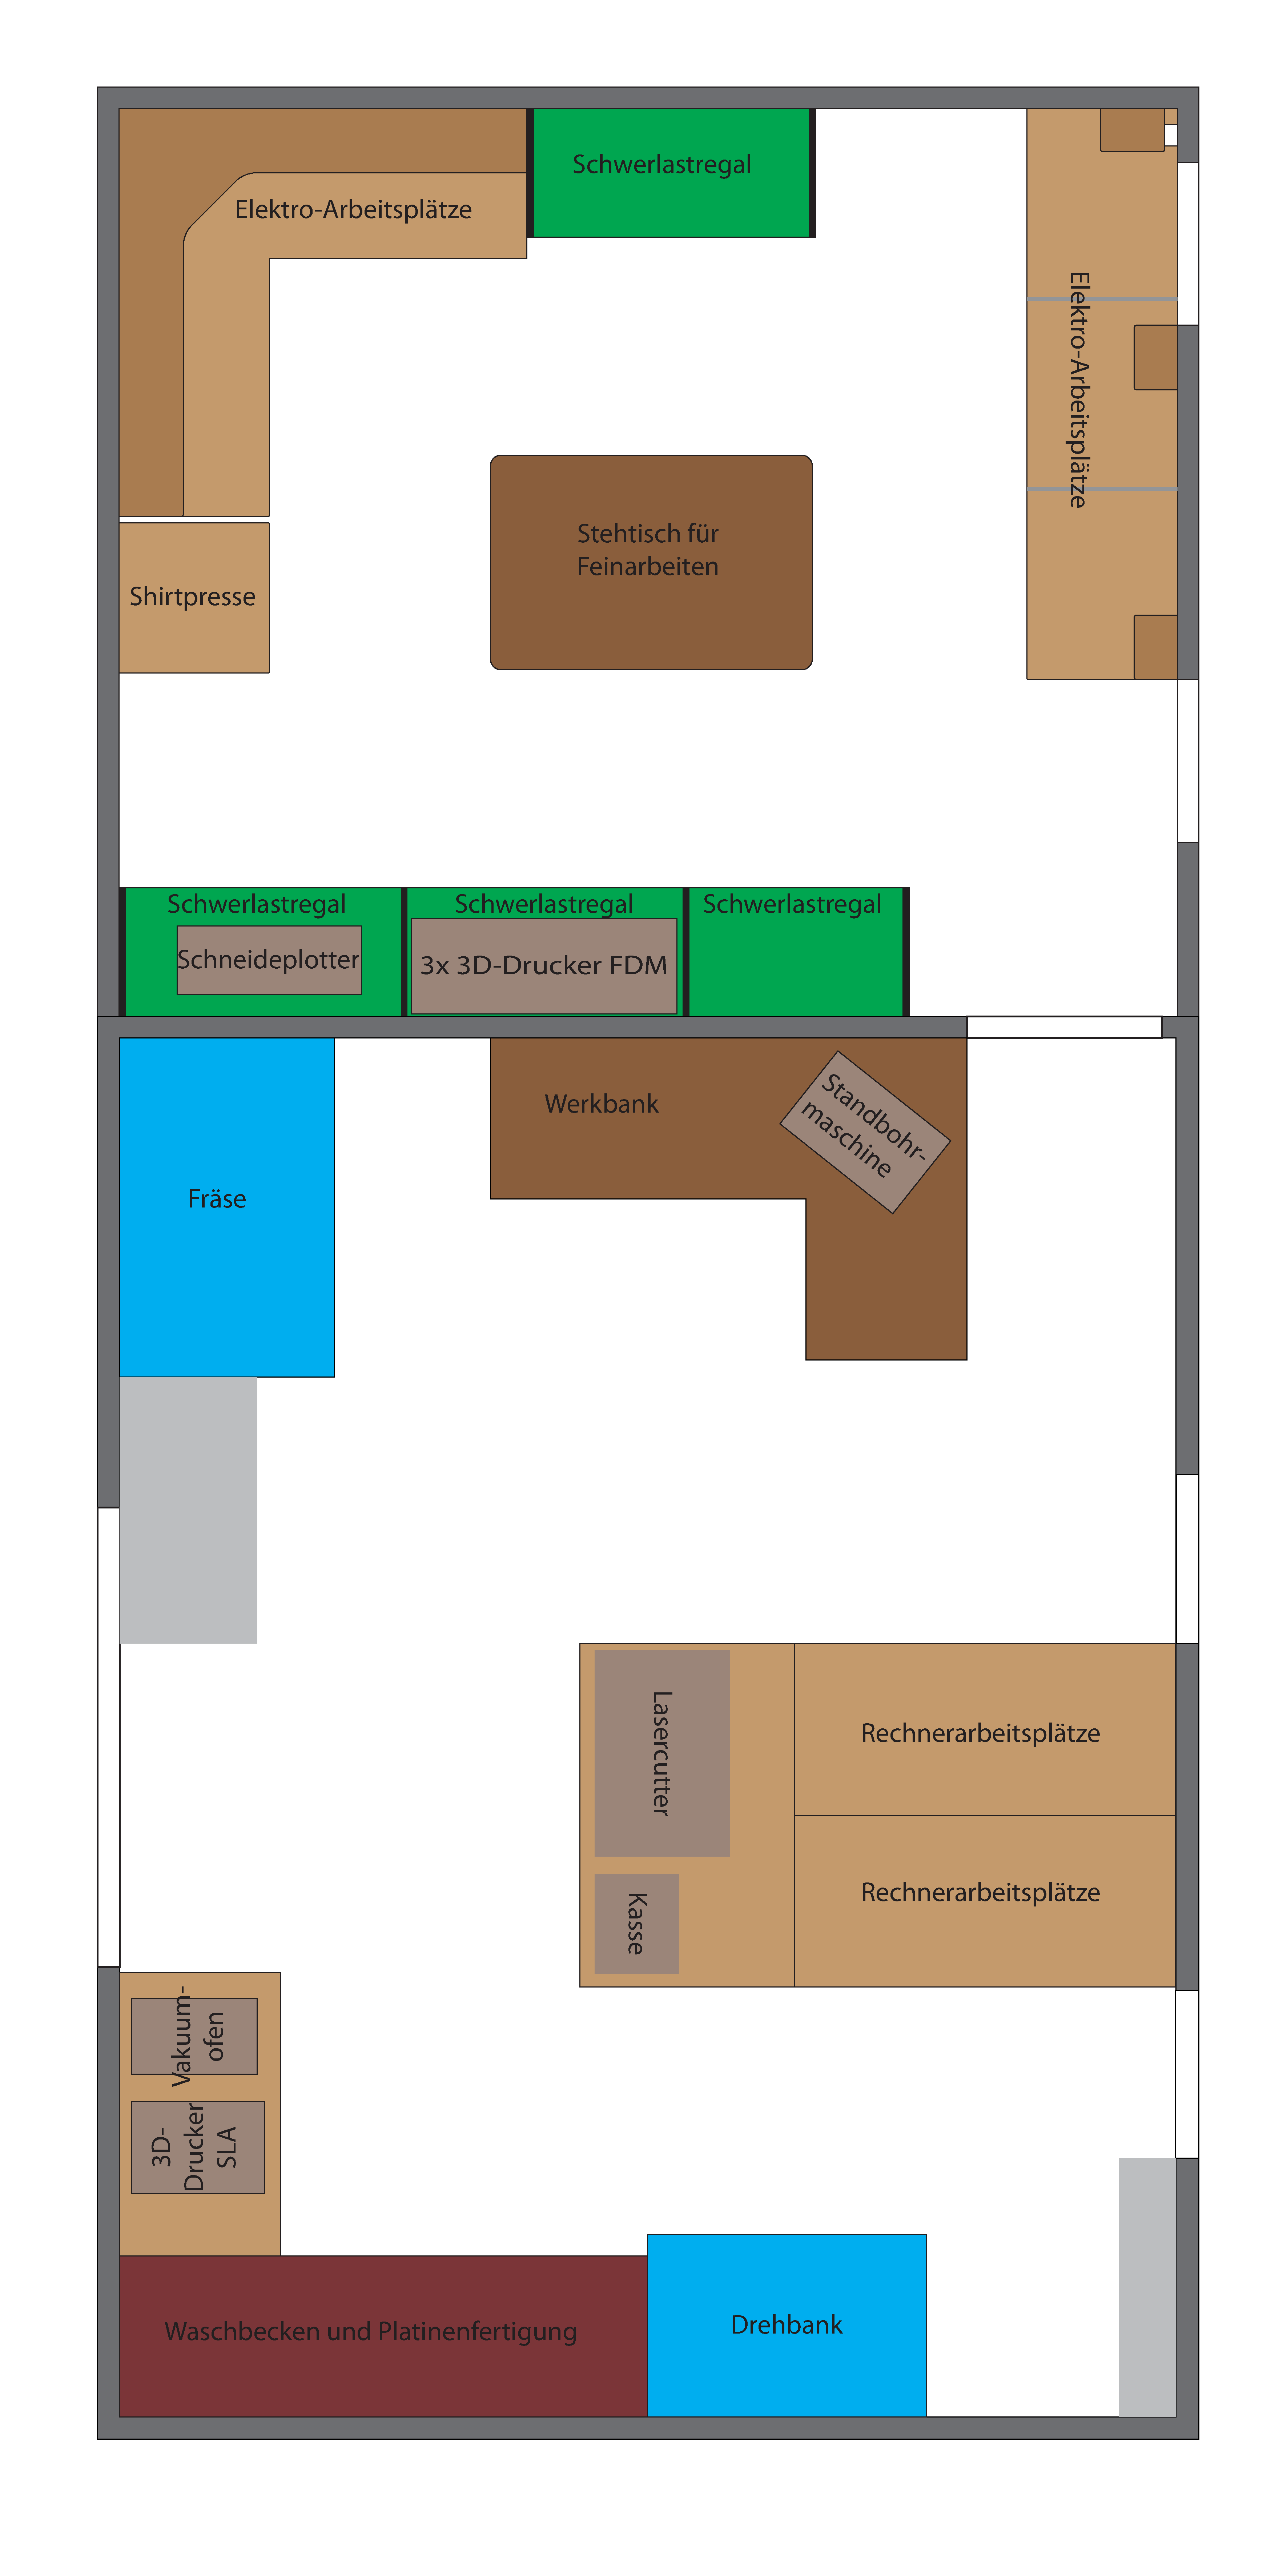
\includegraphics[height=0.9\textheight]{../img/fablabplan.pdf}
        \end{column}
        \begin{column}[T]{0.7\textwidth}
            \includegraphics[width=\textwidth,clip,trim=4cm 3cm 0cm 13cm]{../img/ewerkstatt.jpg}\\
            \includegraphics[width=\textwidth,clip,trim=0cm 5cm 0cm 7cm]{../img/hauptraum.jpg}
        \end{column}
    \end{columns}
\end{frame}

\begin{frame}
    \frametitle{Lasercutter: Cut and Engrave (within seconds)}
    \begin{itemize}
        \item Materials (in-stock): Acrylic, Plywood, MDF, Cardboard
        \item Max workpiece size: 60$\times$30\,cm, up to 10\,mm thickness, accuracy around 0.2\,mm
        \item Vector files (Inkscape, Corel Draw, Illustrator, CAD (.DXF), ...)
    \end{itemize}

    \bigskip

    \bigskip
    \begin{center}
        
\includegraphics[height=6cm]{../img/SquareGears.pdf}
        
\includegraphics[height=6cm]{../img/pfeil.pdf}
        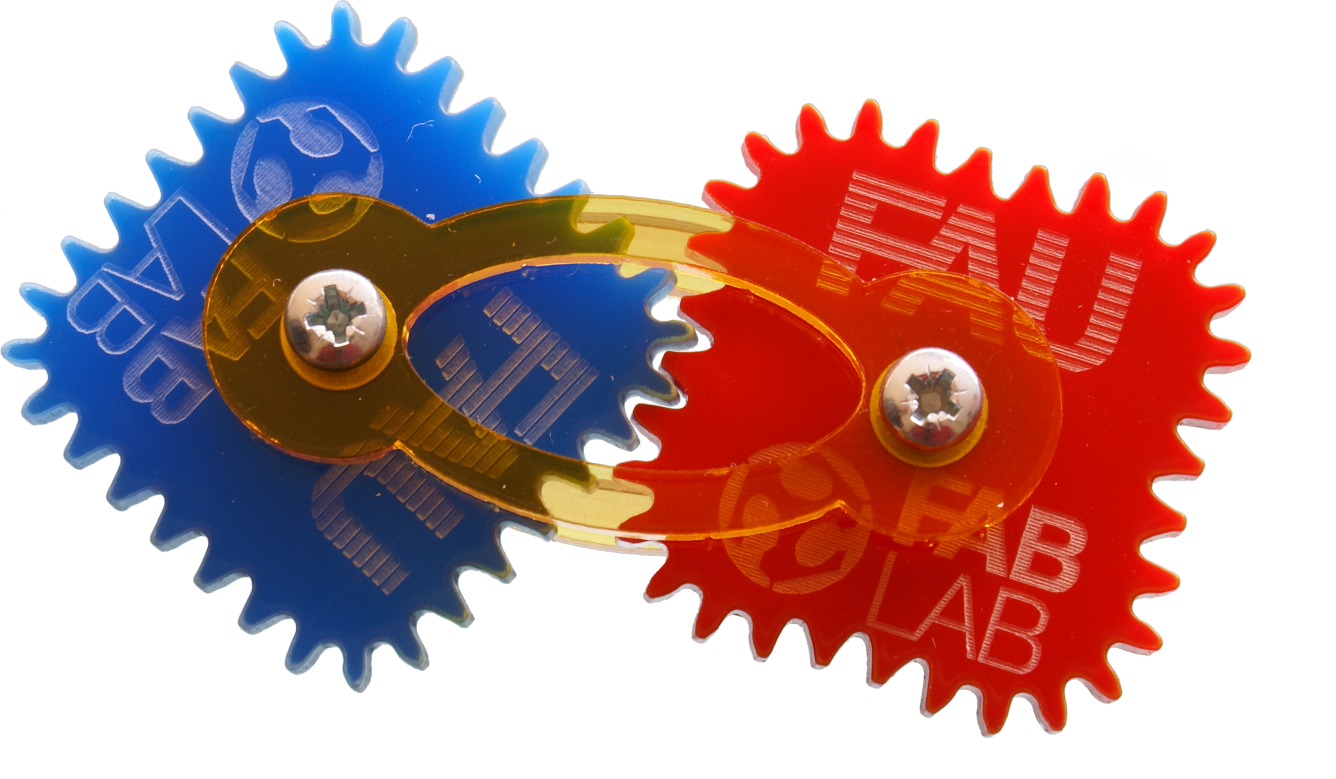
\includegraphics[height=6cm]{../img/zahnraeder2b-skaliert.png}
    \end{center}

\end{frame}


\begin{frame}{Lasercutter: Wood}
    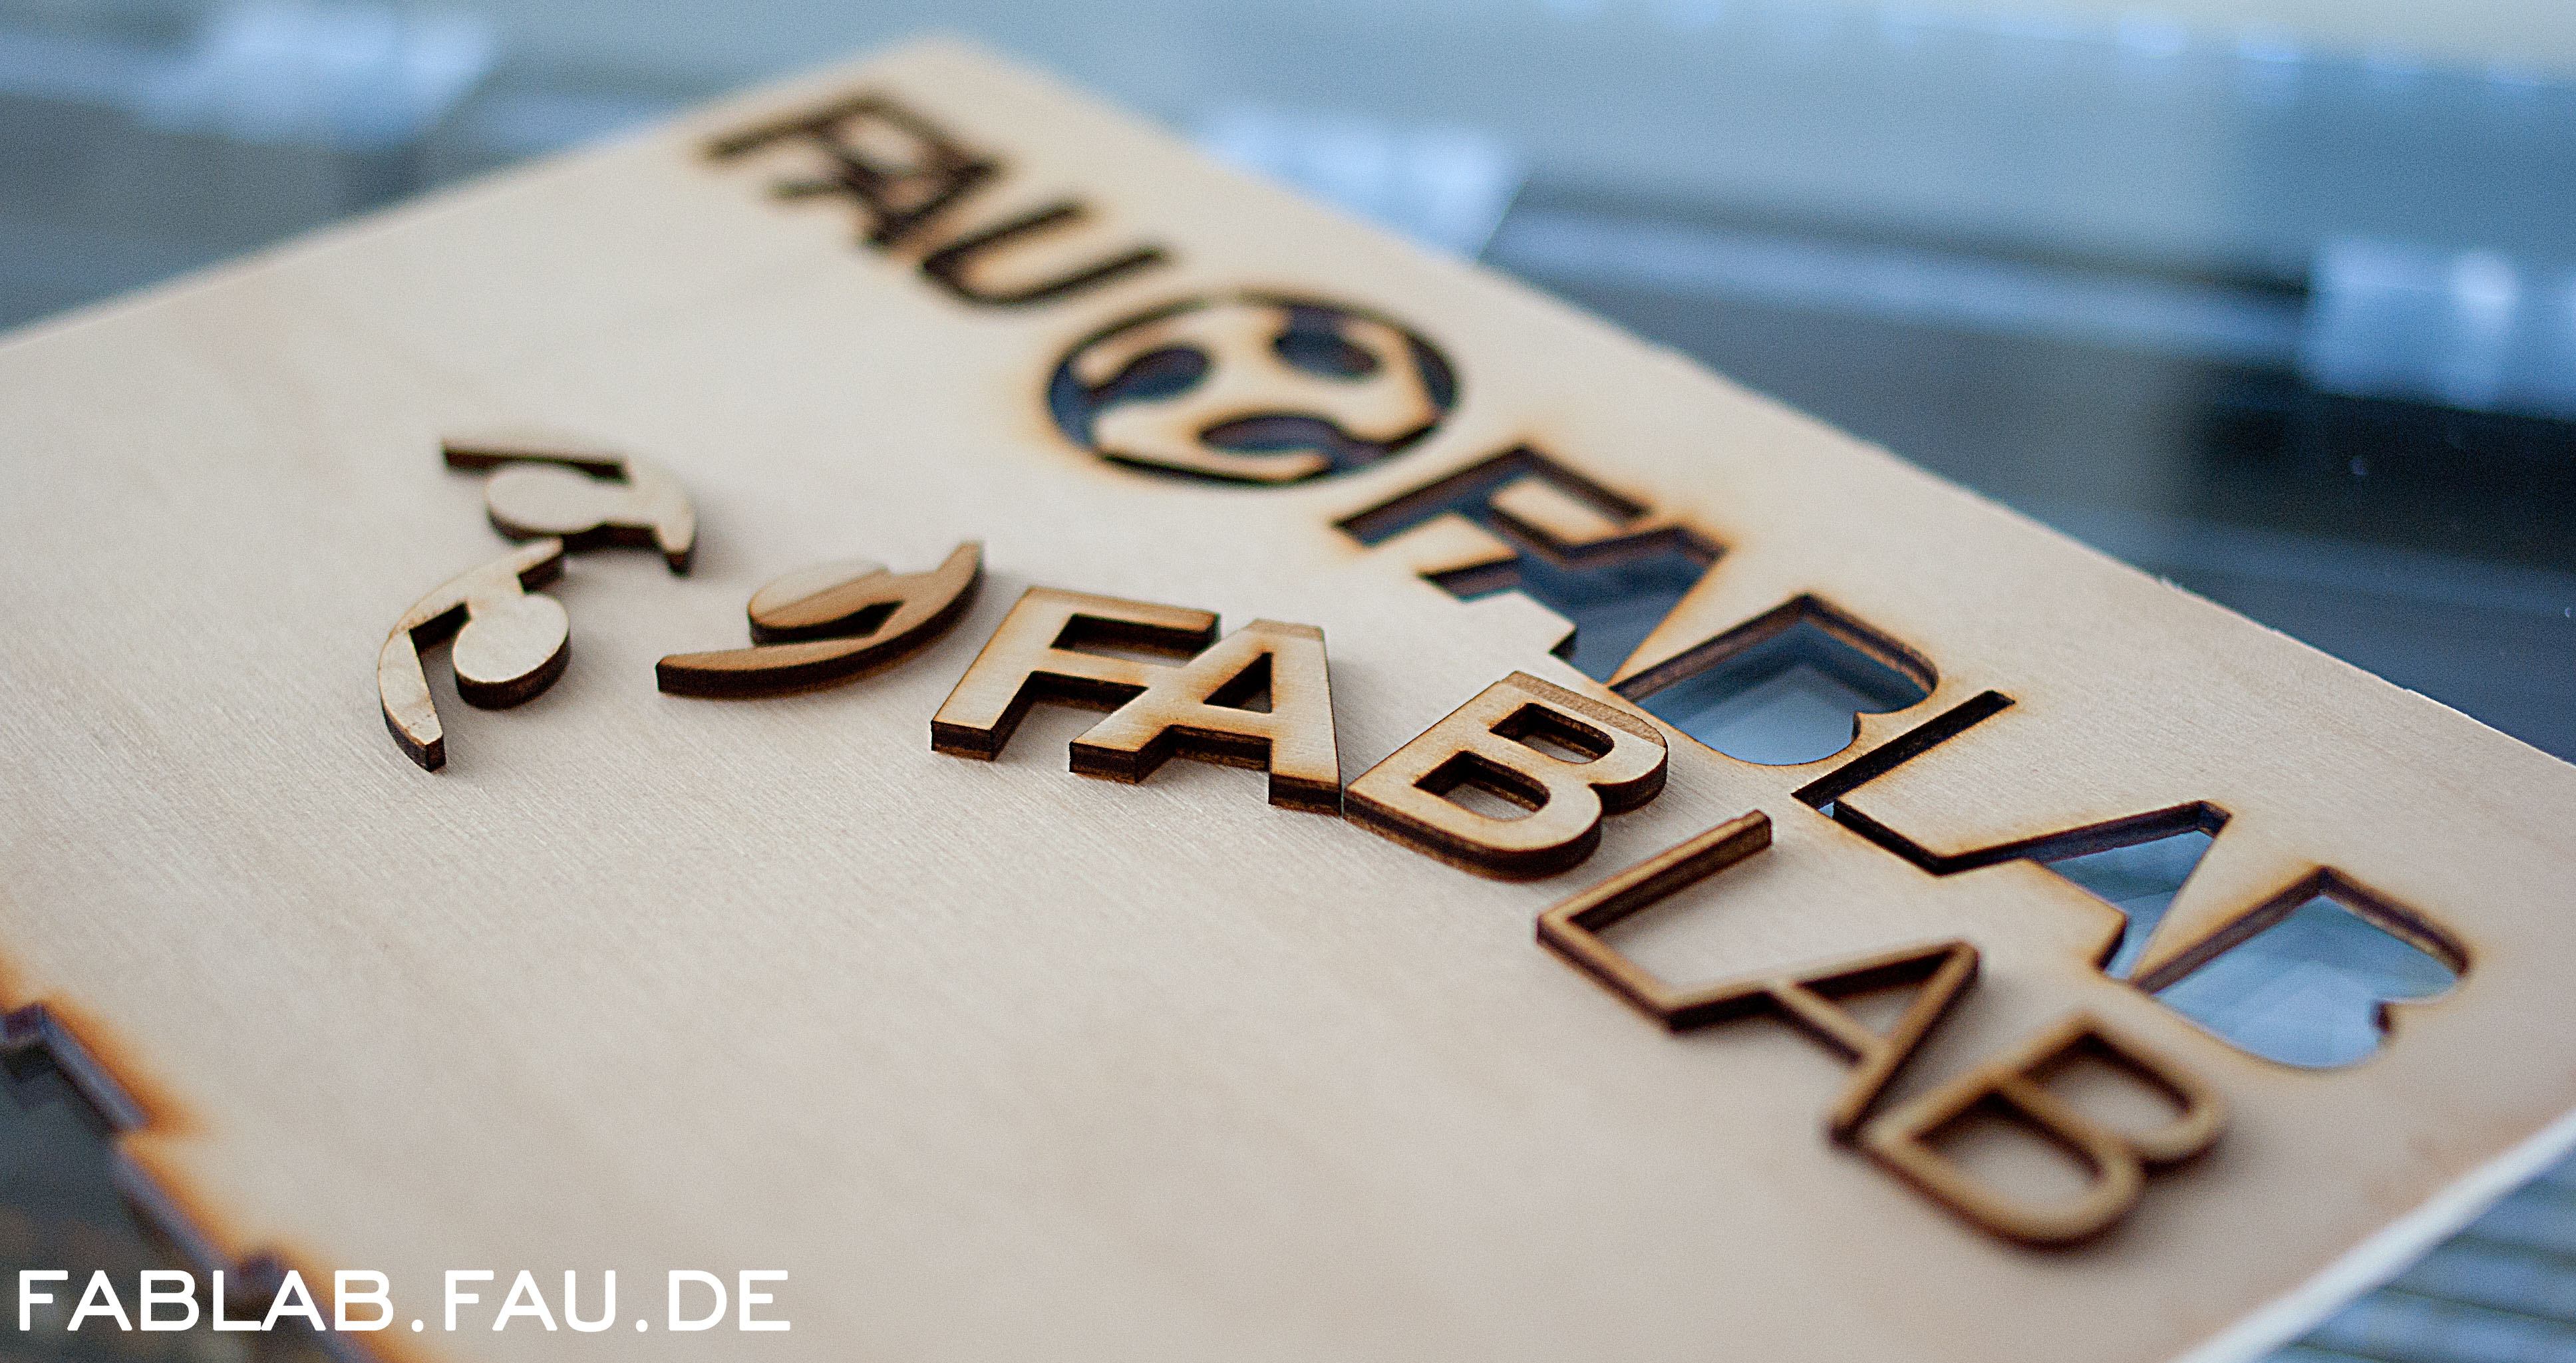
\includegraphics[width=\textwidth]{../img/lasercut-holz.jpg}
\end{frame}
\begin{frame}{Lasercutter: Acrylic}
    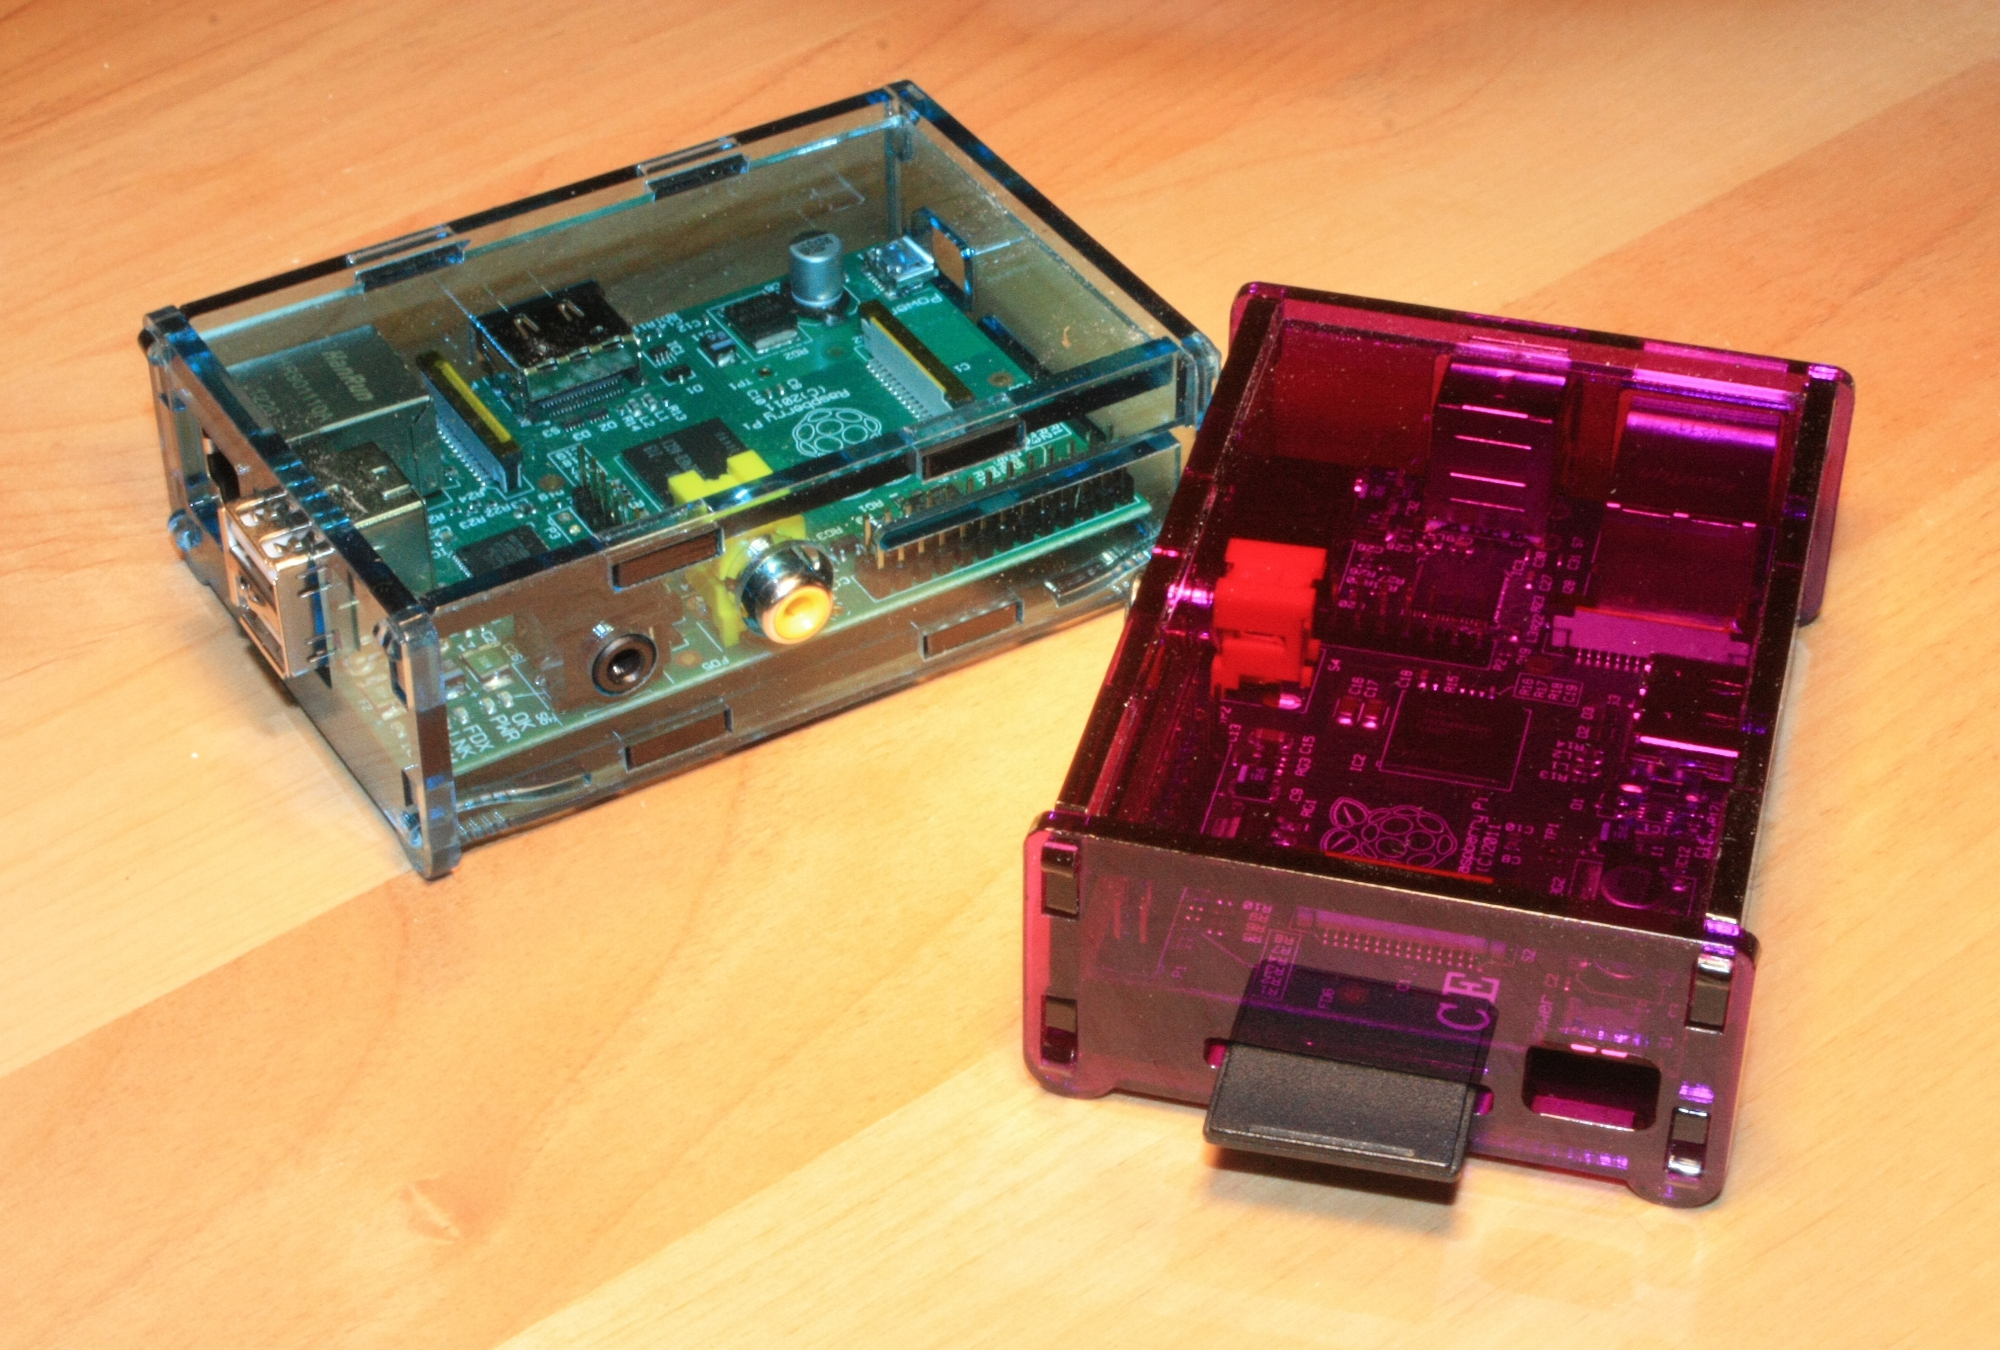
\includegraphics[width=\textwidth,clip,trim=0 5cm 0 2cm]{../img/lasercut-kunststoff.jpg}
\end{frame}

\begin{frame}
    \frametitle{3D-Printer: From CAD to Reality (within hours)}
    \begin{itemize}
        \item Material: PLA or ABS
        \item Maximum size roughly 20$\times$20$\times$20\,cm
        \item Not everything is printable -- ask us!
        \item 3D model files in STL format
    \end{itemize}
    \begin{center}
    ~\\
        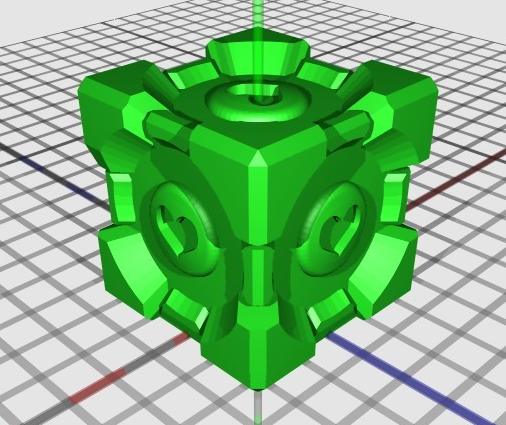
\includegraphics[height=6cm]{../img/companioncube_render.png}
        
\includegraphics[height=6cm]{../img/pfeil.pdf}
        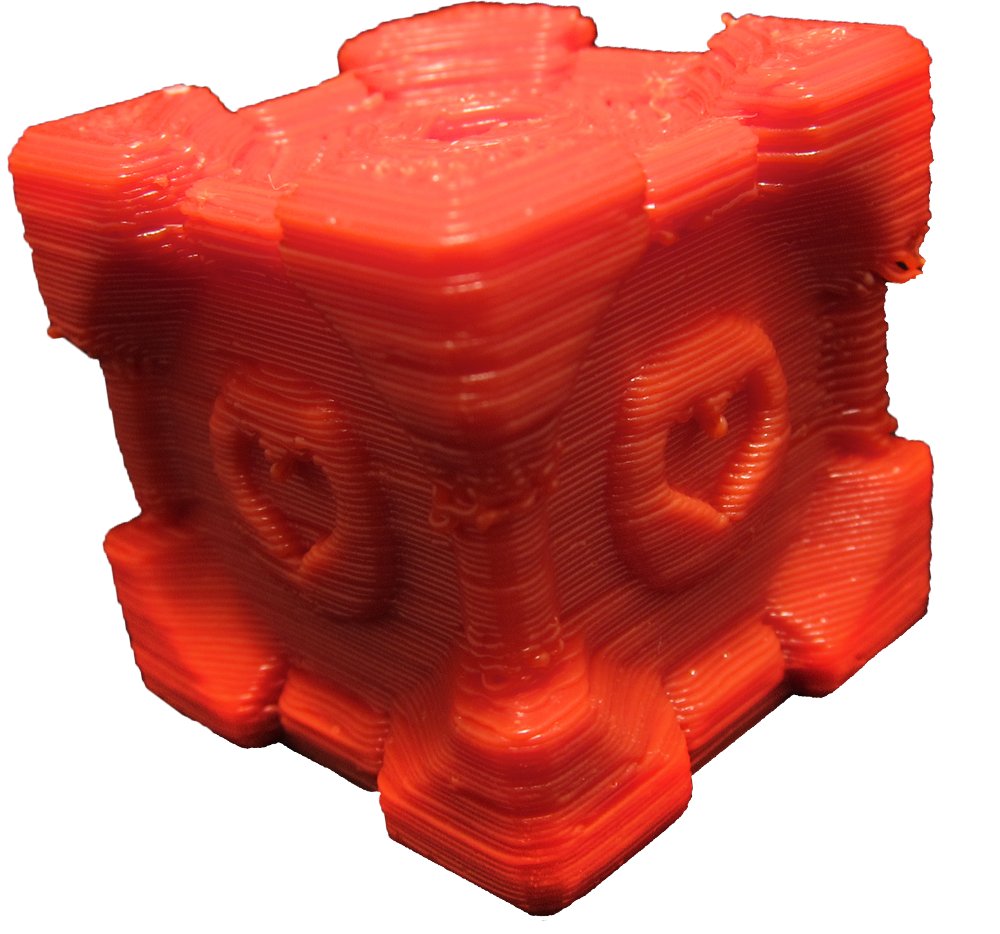
\includegraphics[height=6cm]{../img/companioncube.png}
    \end{center}
\end{frame}

\begin{frame}
    \frametitle{CNC Mill}
    \begin{itemize}
        \item Material: Aluminium, Steel, Wood, Plastics
        \item Work piece up to 50$\times$30$\times$10\,cm
        \item 2D drawing (e.g., DXF) or 3D CAD model (e.g., STEP)
        \item Check producibility with {\color{blue} zerspanung@fablab.fau.de}
    \end{itemize}
    \begin{center}
    ~\\
    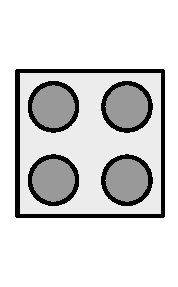
\includegraphics[height=6cm]{../img/legozeichnung.pdf}
    
\includegraphics[height=6cm]{../img/pfeil.pdf}
    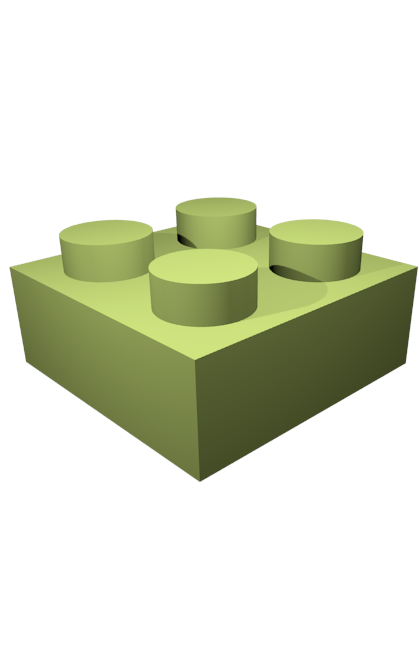
\includegraphics[height=6cm]{../img/fraese-lego-3d.png}
    
\includegraphics[height=6cm]{../img/pfeil.pdf}
    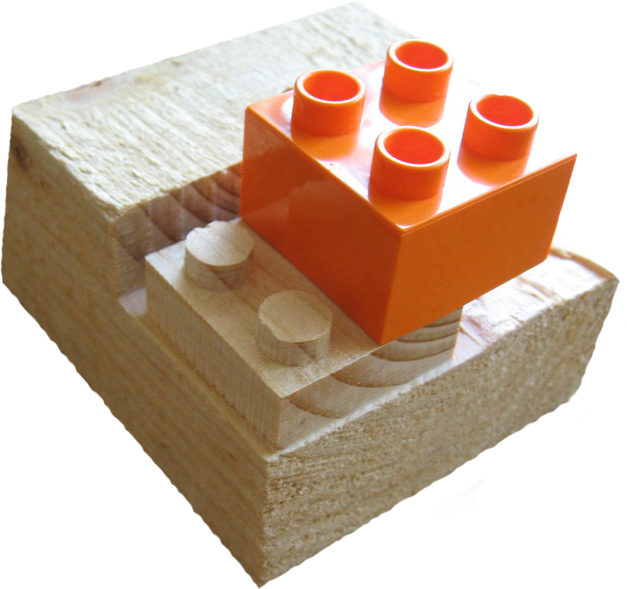
\includegraphics[height=6cm]{../img/fraese-lego.png}

    \end{center}
\end{frame}

\begin{frame}
    \frametitle{Electronics Workbenches}
    \begin{itemize}
        \item Soldering irons, oscilloscopes et cetera
        \item Circuit board etching:\\
            16$\times$10\,cm, single and double sided -- check design rules
        \item Sale of components (about 350 typical components in stock)
    \end{itemize}
        \begin{center}
    ~\\
        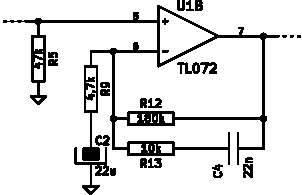
\includegraphics[height=6cm]{../img/schaltplan.pdf}
        
\includegraphics[height=6cm]{../img/pfeil.pdf}
        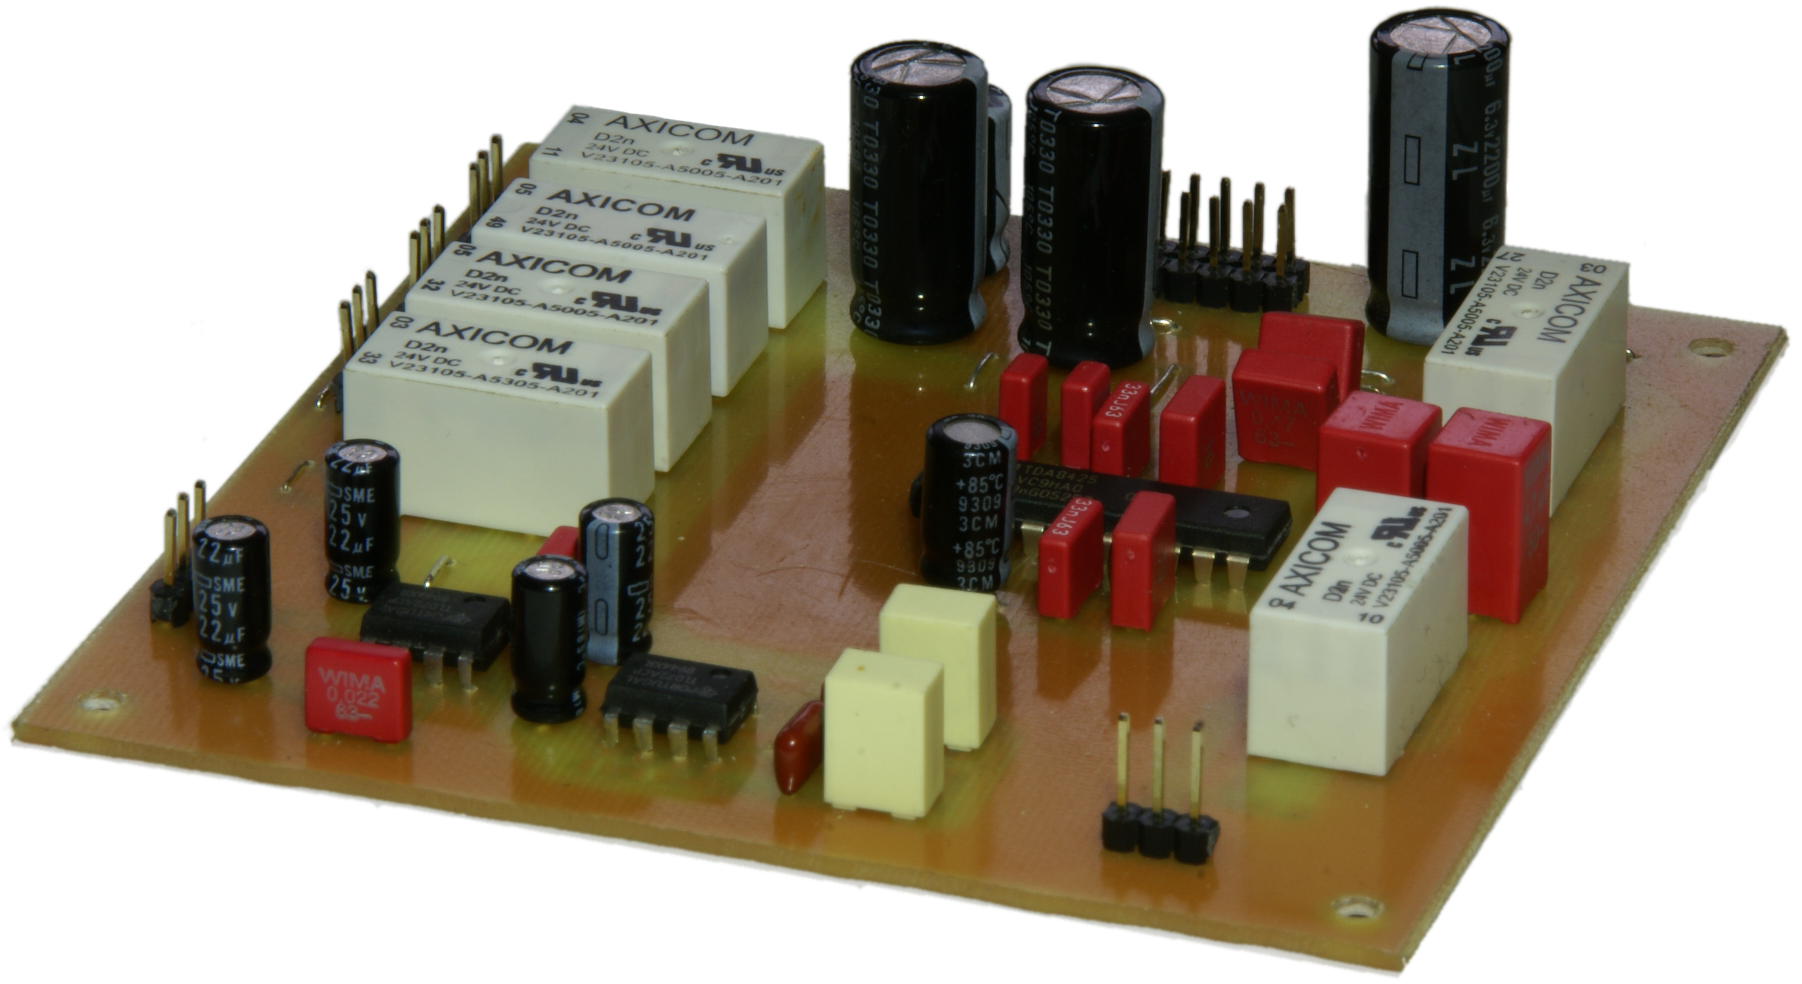
\includegraphics[height=6cm]{../img/platine_perspektivisch.png}
    \end{center}
\end{frame}

\begin{frame}
    \frametitle{and much much more}
    \begin{itemize}
        \item Vinyl cutter
        \item Sewing machine
        \item T-Shirts printing and embroidery
        \item Bike repair rack and compressed-air
        \item CNC lathe
        \item ...
    \end{itemize}
    \begin{center}
        ~\\

        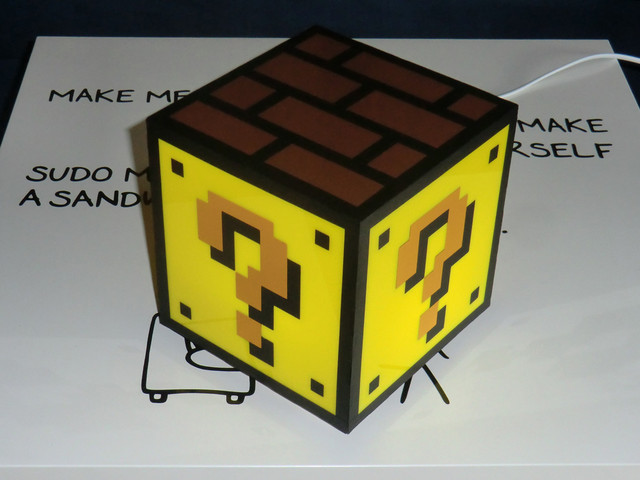
\includegraphics[height=7cm]{../img/mariolampe.jpg}
        \hspace{1em}
        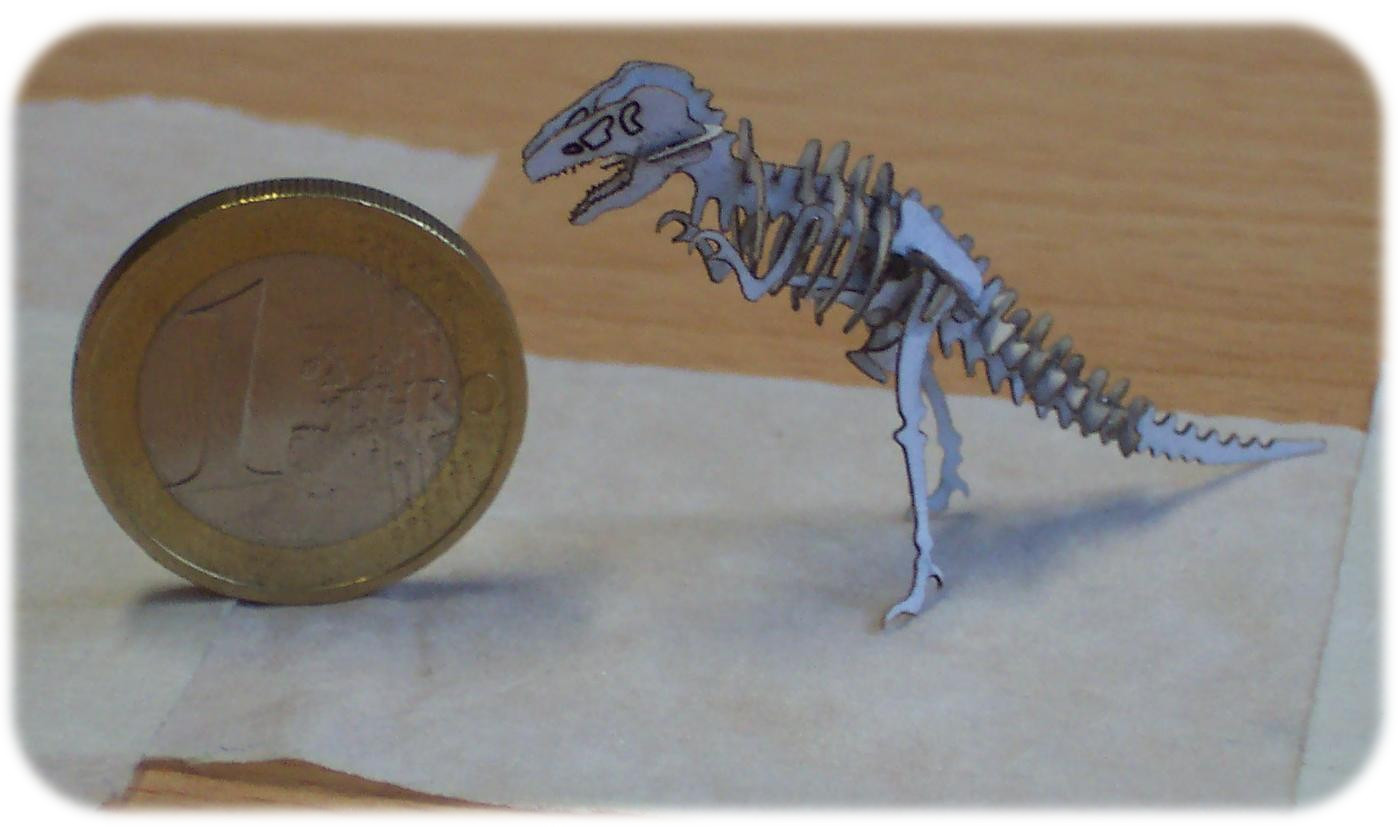
\includegraphics[height=7cm]{../img/tinysaur.jpg}
    \end{center}
\end{frame}

\begin{frame}
    \frametitle{Sparked Your Interest?}

    \begin{itemize}
        \item Where: Lecture hall building, at lower exits of H8/H9 (Erwin-Rommel-Straße 60, Room U1.239)
        \item When: regular OpenLabs starting next week
        % \item Workshops: Löten (Anfänger/Fortgeschrittene), 3D-Modellierung, usw.
        \item Check time table at {\color{blue} https://fablab.fau.de/termine}
    \end{itemize}
%     ~\\
%     Merchandising
%     \begin{itemize}
%         \item Mitgebrachte Werkstücke ansehen
%         \item Flyer mitnehmen
%     \end{itemize}
    ~\\
    Questions?
    \begin{itemize}
        \item Website {\color{blue} https://fablab.fau.de}
        \item Mail {\color{blue} kontakt@fablab.fau.de}
        \item Come by and get inspired
    \end{itemize}
\end{frame}

\end{document}
